% Graphics for slide 15, in the order the PDF draws them.
\begin{tikzpicture}[remember picture, overlay, x=1bp, y=-1bp,
  shift={(current page.north west)}]
\path[fill=cFFFFFF] (0,0) rectangle (960,540);
\node[anchor=north west, inner sep=0pt] at (56.69,477.21) {
\includegraphics[width=73.42bp, height=37.42bp]{figures/fundamentals-of-hpc/p03-1.png}};
\path[fill=cEE7628,even odd rule] (57.18,55.73) ..controls(57.96,55.73)and(58.6,56.37)..(58.6,57.15) --(58.6,85.5) ..controls(58.6,86.28)and(57.96,86.91)..(57.18,86.91) ..controls(56.4,86.91)and(55.76,86.28)..(55.76,85.5) --(55.76,57.15) ..controls(55.76,56.37)and(56.4,55.73)..(57.18,55.73);
\node[anchor=north west, inner sep=0pt] at (241.76,86.91) {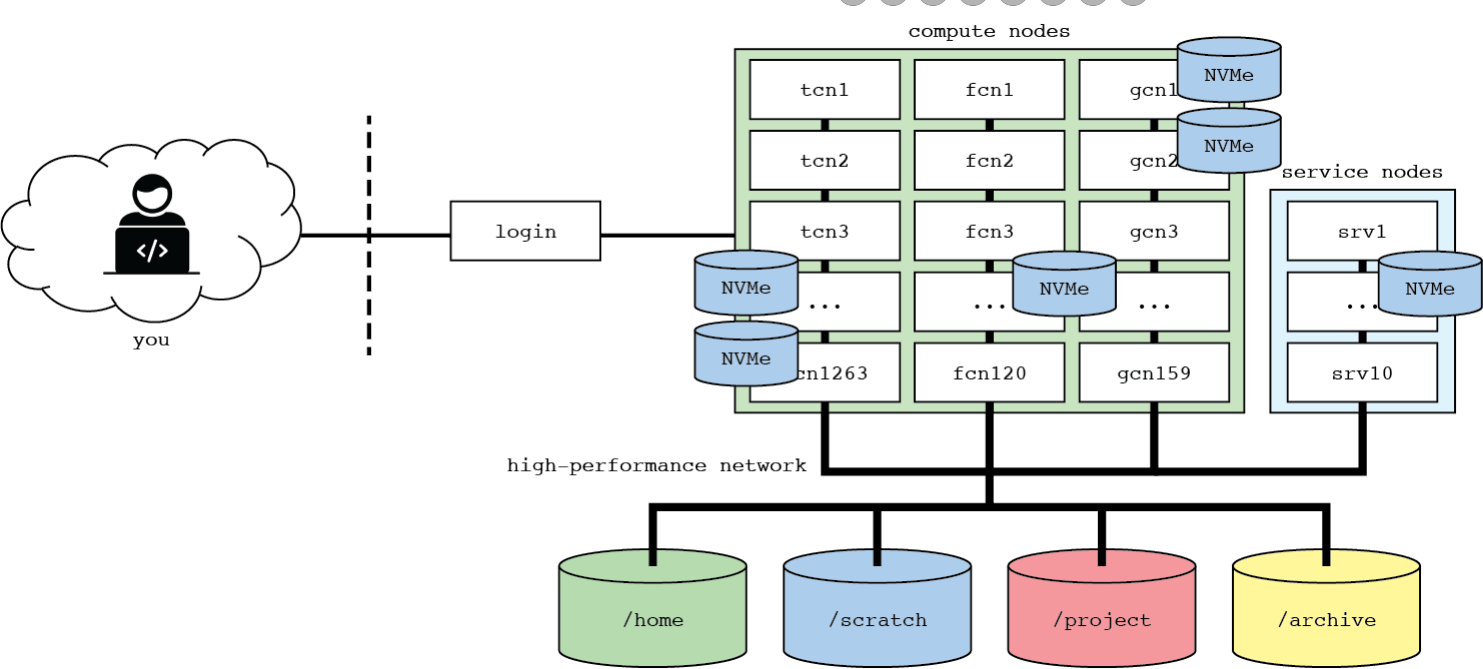
\includegraphics[width=675.46bp, height=304.43bp]{figures/fundamentals-of-hpc/p15-2.png}};
\path[fill=cEA7600] (173.79,422.18) --(169.81,422.18) ..controls(169,422.18)and(168.34,421.53)..(168.34,420.74) --(168.34,418.51) ..controls(168.34,417.71)and(169,417.07)..(169.81,417.07) --(173.79,417.07) ..controls(174.6,417.07)and(175.25,417.71)..(175.25,418.51) --(175.25,420.74) ..controls(175.25,421.53)and(174.6,422.18)..(173.79,422.18);
\path[fill=cEA7600] (173.79,453.38) --(169.81,453.38) ..controls(169,453.38)and(168.34,452.73)..(168.34,451.94) --(168.34,449.71) ..controls(168.34,448.91)and(169,448.27)..(169.81,448.27) --(173.79,448.27) ..controls(174.6,448.27)and(175.25,448.91)..(175.25,449.71) --(175.25,451.94) ..controls(175.25,452.73)and(174.6,453.38)..(173.79,453.38);
\path[fill=cEA7600] (173.79,484.58) --(169.81,484.58) ..controls(169,484.58)and(168.34,483.93)..(168.34,483.14) --(168.34,480.91) ..controls(168.34,480.11)and(169,479.47)..(169.81,479.47) --(173.79,479.47) ..controls(174.6,479.47)and(175.25,480.11)..(175.25,480.91) --(175.25,483.14) ..controls(175.25,483.93)and(174.6,484.58)..(173.79,484.58);
\path[fill=cEA7600] (173.79,515.78) --(169.81,515.78) ..controls(169,515.78)and(168.34,515.13)..(168.34,514.34) --(168.34,512.11) ..controls(168.34,511.31)and(169,510.67)..(169.81,510.67) --(173.79,510.67) ..controls(174.6,510.67)and(175.25,511.31)..(175.25,512.11) --(175.25,514.34) ..controls(175.25,515.13)and(174.6,515.78)..(173.79,515.78);
\node[anchor=north west, inner sep=0pt] at (621.43,7.62) {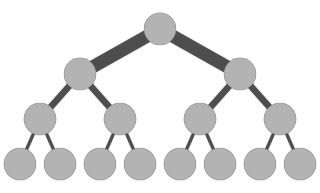
\includegraphics[width=145.45bp, height=87.29bp]{figures/fundamentals-of-hpc/p15-3.png}};
\end{tikzpicture}
